% !TeX root = ../main.tex

\chapter{System Modelling and Problem Formulation}\label{chapter:system-modelling}

In this chapter, the multi-prosumer building energy management problem investigated in this thesis is defined, and the physical models and mathematical formulations involved in the environment are presented. The system under study consists of three prosumers connected to a low-voltage distribution network. Each prosumer is equipped with local electrical loads, PV generation, a stationary battery energy storage system, and residential EV charging demand. At each discrete time step, the control system determines the battery charging/discharging power, PV utilization, and EV charging power to minimize the total electricity purchasing cost while satisfying both the physical constraints of different devices and the safety constraints of the distribution network.
% 本章定义本文研究的多产消者建筑能源管理问题，并介绍仿真环境所涉及的物理模型与数学表达。研究系统由接入低压配电网的三个产消者构成，每个产消者均配置本地用电负荷、光伏发电、固定式电池储能系统以及住宅电动汽车充电需求。在每个离散时间步，控制系统决定电池充放电功率、光伏利用率和电动汽车充电功率，以在满足各类设备物理约束和配电网安全约束的同时，最小化总购电成本。

This chapter focuses only on the system modeling and problem formulation, including the system constraints and the optimization objective function. The details of the control methodology, such as how MADRL actions are generated, how the EV control strategies are implemented at the control layer, and how the grid safety projection modifies the control actions, are discussed in Chapter4.
% 本章仅关注系统建模与问题构建，包括系统约束和优化目标函数。MADRL 动作如何生成、电动汽车控制策略如何在控制层实现，以及电网安全投影如何修正控制动作等具体控制方法，将在第 4 章中讨论。

\section{Overall System}

The system investigated in this thesis addresses the energy management problem of a low-voltage distribution network integrated with distributed energy resources. The system consists of a low-voltage distribution network, 3 prosumer agents, household loads, PV generation, a stationary battery energy storage system, EV charging, electricity price signals, and a power flow calculation module. Each prosumer acts not only as an electricity consumer but also as an electricity producer and the owner of dispatchable energy resources. The primary objective of the system is to coordinate the resources of the three prosumers to minimize the overall operating cost while satisfying both the device operational constraints and the distribution network safety constraints.
% 本文研究集成分布式能源资源的低压配电网能源管理问题。系统由低压配电网、三个产消者智能体、家庭用电负荷、光伏发电、固定式电池储能系统、电动汽车充电、电价信号和潮流计算模块组成。每个产消者不仅是电力消费者，也是电力生产者和可调度能源资源的拥有者。系统的主要目标是协调三个产消者的资源，在满足设备运行约束和配电网安全约束的同时，最小化总体运行成本。

The distribution network topology is adopted from SimBench, with the fixed network configuration:
% 配电网拓扑采用 SimBench 中的以下固定网络配置：
\[
  \texttt{1-LV-rural1--0-sw}.
\]

The system consists of \(N=3\) prosumers connected to the distribution network buses
% 系统包含 \(N=3\) 个产消者，分别接入以下配电网母线：
\[
  \mathcal{B} = \{12,4,2\}.
\]
Let \(i\in\mathcal{I}=\{1,2,3\}\) denote the prosumer index, and \(t\in\mathcal{T}=\{0,\ldots,T-1\}\) represent the discrete time step within an episode. The simulation uses a 15-minute resolution, so a day is represented as:
% 令 \(i\in\mathcal{I}=\{1,2,3\}\) 表示产消者索引，\(t\in\mathcal{T}=\{0,\ldots,T-1\}\) 表示一个回合内的离散时间步。仿真采用 15 分钟时间分辨率，因此一天可表示为：
\[
  \Delta t = 0.25\ \mathrm{h}, \qquad T=96.
\]

One episode corresponds to the operation of one whole day. During training, multiple consecutive days can be concatenated to form a longer training window.
% 一个回合对应完整一天的运行过程。在训练期间，可以将多个连续日拼接起来形成更长的训练窗口。

% Modified: use the general aggregated-load notation here; the load components and their numerical settings are specified in Chapter 5.
The local power profile of each prosumer \(i\) consists of external inputs and three kinds of controllable or semi-controllable energy resources. The external inputs include the aggregated electrical demand \(L_{i,t}\), the available PV generation \(G_{i,t}\), and the electricity price \(p_t\). The aggregated demand may contain several exogenous load components, whose general formulation is introduced in Section~\ref{sec:prosumer-load}; the component selection and numerical settings used in the experiments are reported in Chapter~\ref{chapter:experimental-setup}.
% 可控资源包括 stationary battery 的充放电功率 \(P^b_{i,t}\)、PV实际利用功率 \(G^{use}_{i,t}\) 以及 EV 充电功率 \(P^{ev}_{i,t}\)。因此每个 prosumer 的电相关变量可以概括为
The controllable resources include the charging and discharging power of the stationary battery \(P^b_{i,t}\), the utilized PV generation \(G^{use}_{i,t}\), and the EV charging power \(P^{ev}_{i,t}\). Accordingly, the electricity-related variables of each prosumer can be expressed as
% 可控资源包括固定式电池充放电功率 \(P^b_{i,t}\)、实际利用的光伏发电功率 \(G^{use}_{i,t}\) 以及电动汽车充电功率 \(P^{ev}_{i,t}\)。因此，每个产消者的电力相关变量可表示为：
\[
  \{L_{i,t},\ G_{i,t},\ P^{b}_{i,t},\ P^{ev}_{i,t}\},
\]
% 其中 \(L_{i,t}\) 为本地总负荷，\(G_{i,t}\) 为可用 PV 功率，\(P^{b}_{i,t}\) 为静态电池功率，\(P^{ev}_{i,t}\) 为 EV 充电功率。本文采用如下功率符号约定：\(P^{b}_{i,t}>0\) 表示电池充电，\(P^{b}_{i,t}<0\) 表示电池放电。
where \(L_{i,t}\) denotes the total local electrical load, \(G_{i,t}\) denotes the available PV generation, \(P^{b}_{i,t}\) denotes the stationary battery power, and \(P^{ev}_{i,t}\) denotes the EV charging power. In this thesis, \(P^{b}_{i,t}>0\) indicates battery charging, whereas \(P^{b}_{i,t}<0\) indicates battery discharging.
% 其中，\(L_{i,t}\) 表示本地总电力负荷，\(G_{i,t}\) 表示可用光伏发电功率，\(P^{b}_{i,t}\) 表示固定式电池功率，\(P^{ev}_{i,t}\) 表示电动汽车充电功率。本文规定 \(P^{b}_{i,t}>0\) 表示电池充电，\(P^{b}_{i,t}<0\) 表示电池放电。
\[
  -P^{b,\max}_i \le P^b_{i,t} \le P^{b,\max}_i.
\]
% EV 只考虑充电，不考虑 vehicle-to-grid 放电，因此
Since only EV charging is considered in this thesis, while vehicle-to-grid is not allowed, the EV charging power satisfies
% 由于本文仅考虑电动汽车充电且不允许车辆到电网放电，电动汽车充电功率满足：
\[
  P^{ev}_{i,t}\ge 0.
\]

At each time step, the power of all devices within a prosumer is aggregated to determine the net load injected into the distribution network:
% 在每个时间步，将产消者内部所有设备的功率汇总，以确定注入配电网的净负荷：
\[
  P^{net}_{i,t}
  =
  L_{i,t}
  -
  G^{use}_{i,t}
  +
  P^b_{i,t}
  +
  P^{ev}_{i,t}.
\]
% 当 \(P^{net}_{i,t}>0\) 时，该 prosumer 从电网取电；当 \(P^{net}_{i,t}<0\) 时，该 prosumer 向电网反送功率。三个 prosumer 的净负荷共同写入低压配电网模型，并通过 pandapower 执行潮流计算。潮流计算返回母线电压、线路负载率和变压器负载率，这些量用于判断控制动作是否满足电网安全要求。
When \(P^{net}_{i,t}>0\), the prosumer imports electricity from the distribution grid; when \(P^{net}_{i,t}<0\), the prosumer exports power back to the grid. The net loads of the three prosumers are injected into the low-voltage distribution network model, where power flow analysis is performed using pandapower. The power flow calculation returns the bus voltages, line loading ratios, and transformer loading ratios, which are subsequently used to determine whether the control actions satisfy the distribution network safety constraints.
% 当 \(P^{net}_{i,t}>0\) 时，产消者从配电网购电；当 \(P^{net}_{i,t}<0\) 时，产消者向电网反送功率。三个产消者的净负荷被注入低压配电网模型，并使用 pandapower 进行潮流分析。潮流计算返回母线电压、线路负载率和变压器负载率，随后利用这些结果判断控制动作是否满足配电网安全约束。

\begin{figure}[htbp]
  \centering
  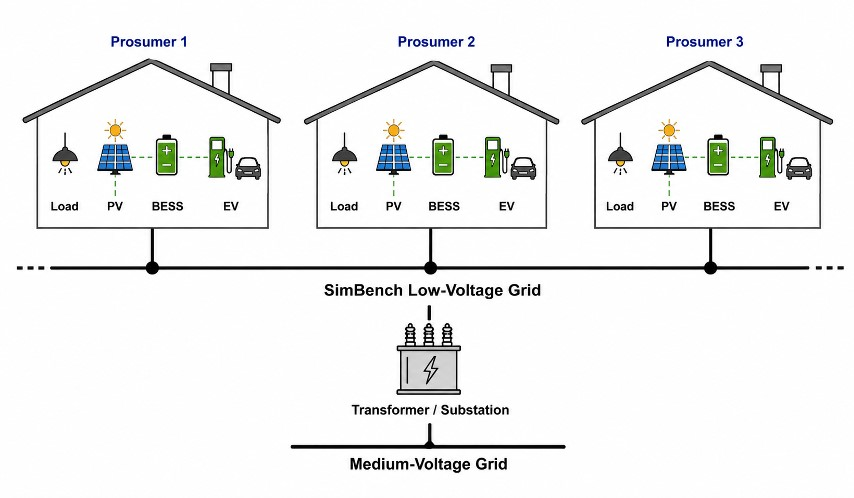
\includegraphics[width=0.95\textwidth]{figures/system_overview.jpg}
  \caption{Overall architecture of the system investigated in this thesis.}
  \label{fig:system-overview}
\end{figure}

Figure~\ref{fig:system-overview} illustrates the overall architecture of the system. The household load, PV generation, and electricity price are treated as time-series inputs from the dataset. The stationary battery and EV charging serve as the dispatchable resources on the prosumer side. The grid power flow calculation module maps the net load of each prosumer to the corresponding network operating states, including bus voltages and equipment loading conditions. Accordingly, the problem addressed in this thesis can be formulated as follows: at each discrete time step, the control system determines \(P^b_{i,t}\), \(G^{use}_{i,t}\), and \(P^{ev}_{i,t}\) for each prosumer based on the load demand, PV generation, electricity price, and the state of charge of the energy storage devices, with the objective of minimizing the total cost while ensuring the safe operation of the stationary battery, the EV, and the distribution network.
% 图~\ref{fig:system-overview} 展示了系统的总体架构。家庭用电负荷、光伏发电和电价由数据集以时间序列输入形式提供，固定式电池和电动汽车充电则作为产消者侧的可调度资源。电网潮流计算模块将每个产消者的净负荷映射为相应的网络运行状态，包括母线电压和设备负载情况。因此，本文所研究的问题可表述为：在每个离散时间步，控制系统根据负荷需求、光伏发电、电价以及储能设备的荷电状态，为每个产消者确定 \(P^b_{i,t}\)、\(G^{use}_{i,t}\) 和 \(P^{ev}_{i,t}\)，目标是在确保固定式电池、电动汽车和配电网安全运行的同时，最小化总运行成本。

\section{Load of the Prosumers}\label{sec:prosumer-load}

% Modified: retain only the general load model in Chapter 3 and move dataset paths, selected profiles, time-zone processing, and scale values to Chapter 5.
The exogenous electrical demand of each prosumer can consist of multiple load components. Let \(\mathcal{C}^{L}\) denote the set of load components, and let \(L^{raw}_{c,i,t}\) represent the unscaled demand of component \(c\in\mathcal{C}^{L}\) for prosumer \(i\) at time step \(t\). An agent-specific scaling factor \(s^L_i\) maps the original profile to the demand level considered in the simulation. The aggregated prosumer load is therefore
\[
  L_{i,t}=s^L_i\sum_{c\in\mathcal{C}^{L}}L^{raw}_{c,i,t}.
\]
This formulation allows different electrical demand components and prosumer-specific demand levels to be represented without changing the subsequent battery, EV, PV, or grid equations. The experimental choices for \(\mathcal{C}^{L}\), the selected prosumer profiles, and \(s^L_i\) are specified in Chapter~\ref{chapter:experimental-setup}. The resulting \(L_{i,t}\) represents only exogenous demand; PV generation, stationary-battery power, and EV charging are incorporated separately in the net-load equation.

\section{PV Modelling}

The available PV power is obtained from the data file
% 可用光伏功率取自以下数据文件：
\[
  \texttt{datasets/prosumer/pv\_reference.csv}.
\]
In the current configuration, the reference column \(\mathrm{ref\_south}\) is used. The same reference PV profile is assigned to all three prosumers and scaled by an agent-specific scaling factor \(s^G_i\),
% 当前配置采用参考列 \(\mathrm{ref\_south}\)。三个产消者使用同一条参考光伏曲线，并通过智能体专属缩放系数 \(s^G_i\) 进行缩放：
\[
  s^G_1=s^G_2=s^G_3=1.
\]
Accordingly, the available PV generation is given by
% 因此，可用光伏发电功率为：
\[
  G_{i,t}=s^G_i G^{ref}_t.
\]
The controller does not directly modify the available PV generation \(G_{i,t}\); instead, it determines the utilized PV power \(G^{use}_{i,t}\). Let \(u^{pv}_{i,t}\in[0,1]\) denote the PV utilization factor. Then,
% 控制器不直接修改可用光伏发电功率 \(G_{i,t}\)，而是决定实际利用的光伏功率 \(G^{use}_{i,t}\)。令 \(u^{pv}_{i,t}\in[0,1]\) 表示光伏利用系数，则有：
\[
  G^{use}_{i,t}=u^{pv}_{i,t}G_{i,t},
\]
\[
  G^{curt}_{i,t}=G_{i,t}-G^{use}_{i,t}.
\]
\(G^{curt}_{i,t}\) denotes the curtailed PV power. In the current model, no explicit penalty is assigned to PV curtailment. Therefore, PV curtailment primarily affects the system performance indirectly by changing the net load and the operating state of the distribution network.

\section{Stationary Battery Energy Storage Model}

Each prosumer is equipped with a stationary battery. Let \(C^b_i\) denote the battery capacity, and let \(SOC^b_{i,t}\) denote the battery state of charge (SoC) at the beginning of time step \(t\). The default parameters are
% 每个产消者均配置一个固定式电池。令 \(C^b_i\) 表示电池容量，\(SOC^b_{i,t}\) 表示时间步 \(t\) 开始时的电池荷电状态（SoC）。默认参数为：
\[
  C^b_i=100\ \mathrm{kWh}, \qquad
  SOC^b_{\min}=0.05, \qquad
  SOC^b_{\max}=0.95.
\]
The battery charging and discharging efficiency is
% 电池充放电效率为：
\[
  \eta_b=0.95.
\]
Maximum charging and discharging powers are determined by the capacity and maximum charging rate:
% 最大充电和放电功率由电池容量与最大充电倍率决定：
\[
  P^{b,\max}_i = r^b_{\max} C^b_i,
\]
where the default \(r^b_{\max}=0.5\), thus a 100 kWh battery corresponds to
% 默认设置为 \(r^b_{\max}=0.5\)，因此容量为 \(100\ \mathrm{kWh}\) 的电池对应：
\[
  P^{b,\max}_i=50\ \mathrm{kW}.
\]
The battery power constraints are
% 电池功率约束为：
\[
  -P^{b,\max}_i \le P^b_{i,t} \le P^{b,\max}_i.
\]

The battery SoC dynamics are determined by the charging and discharging directions as mentioned before. The SoC is updated as
% 电池 SoC 动态由上述充放电方向决定。当 \(P^b_{i,t}\ge 0\) 时，电池处于充电状态；当 \(P^b_{i,t}<0\) 时，电池处于放电状态。SoC 更新为：
\[
SOC^b_{i,t+1} =
\left\{
\begin{array}{ll}
SOC^b_{i,t}+\frac{P^b_{i,t}\Delta t\eta_b}{C^b_i},
& P^b_{i,t}\ge 0,\\[2mm]
SOC^b_{i,t}+\frac{P^b_{i,t}\Delta t}{\eta_b C^b_i},
& P^b_{i,t}<0.
\end{array}
\right.
\]
subject to the boundary constraint
% 并满足以下边界约束：
\[
  SOC^b_{\min}\le SOC^b_{i,t+1}\le SOC^b_{\max}.
\]
This formulation shows the charging and discharging efficiency losses. During charging, only a fraction \(\eta_b\) of the input electrical energy is stored in the battery. During discharging, a larger amount of internal battery energy must be consumed to deliver the same amount of electrical energy to the external system.
% 该表达式体现了充放电效率损失的影响。充电时，输入电能中只有比例为 \(\eta_b\) 的部分被存入电池；放电时，为向外部系统输出相同数量的电能，需要消耗更多的电池内部能量。

\section{EV Modelling}

% 每个 prosumer 配置一辆家庭 EV。EV 在配电网模型中表现为一个具有连接时间窗口、功率上限、电池容量和离家 SoC 需求的可控充电负荷。本文不考虑 vehicle-to-grid，因此 EV 不能向建筑或电网放电，只能在车辆连接到家庭充电桩时吸收电能。令 \(C^{ev}_i\) 表示 EV 电池容量，\(SOC^{ev}_{i,t}\) 表示时间步 \(t\) 开始时 EV 的荷电状态。默认参数为
Each prosumer is equipped with one residential EV. In the distribution network model, the EV is represented as a controllable charging load characterized by a connection time window, a charging power limit, a battery capacity, and a required departure SoC. In this thesis, vehicle-to-grid operation is not considered. Therefore, the EV can only draw electrical energy while connected to the residential charger. Let \(C^{ev}_i\) denote the EV battery capacity, and let \(SOC^{ev}_{i,t}\) denote SoC of the EV at the beginning of time step \(t\). The default parameters are
% 每个产消者均配备一辆住宅电动汽车。在配电网模型中，电动汽车被表示为一种可控充电负荷，其特征包括连接时间窗口、充电功率上限、电池容量以及离开时所需 SoC。本文不考虑车辆到电网（V2G）运行，因此电动汽车不能向建筑或配电网放电，只能在接入住宅充电桩期间吸收电能。令 \(C^{ev}_i\) 表示电动汽车电池容量，\(SOC^{ev}_{i,t}\) 表示时间步 \(t\) 开始时的电动汽车荷电状态。默认参数为：
\[
  C^{ev}_i=60\ \mathrm{kWh}, \qquad
  SOC^{ev}_{\min}=0.10, \qquad
  SOC^{ev}_{\max}=0.95.
\]
The maximum power of the residential charger is
% 住宅充电桩的最大功率为：
\[
  P^{ev,\max}_i=11\ \mathrm{kW},
\]
and the EV charging efficiency is
% 电动汽车充电效率为：
\[
  \eta_{ev}=0.95.
\]
% 由于时间步长为 \(\Delta t=0.25\ \mathrm{h}\)，单个 15 分钟时间步内的最大充电能量为
Since the simulation time step is \(\Delta t=0.25\ \mathrm{h}\), the maximum amount of energy that can be charged during a single 15-minute time step is
% 由于仿真时间步为 \(\Delta t=0.25\ \mathrm{h}\)，单个 15 分钟时间步内可充入的最大能量为：
\[
  E^{ev,\max}_{i,\Delta t}
  =
  P^{ev,\max}_i\Delta t\eta_{ev}.
\]

\subsection{EV Connection Window}

EV's connection status is determined by the intraday time steps. The current assumption is that the vehicle arrives home at 18:00 and connects to the residential charger, and departs at 07:00 the next day. Since there are 96 fifteen-minute time steps in a day, the arrival and departure times are
% 电动汽车的连接状态由日内时间步决定。当前假设车辆于 18:00 到家并接入住宅充电桩，于次日 07:00 离开。由于一天包含 96 个 15 分钟时间步，到达和离开时刻为：
\[
  t^{arr}=72,\qquad t^{dep}=28.
\]
Let \(t_d=t\bmod T\) denote the intraday time step. Since \(t^{arr}>t^{dep}\), the connection window spans midnight, and thus a complete parking window consists of the time steps \(72,\ldots,95\) from the evening of the current day and the time steps \(0,\ldots,27\) from the early morning of the next day:
% 令 \(t_d=t\bmod T\) 表示日内时间步。由于 \(t^{arr}>t^{dep}\)，连接窗口跨越午夜，因此一个完整停车窗口由当日晚间的时间步 \(72,\ldots,95\) 和次日清晨的时间步 \(0,\ldots,27\) 组成：
\[
  \mathcal{T}^{ev}
  =
  \{t:t_d\ge t^{arr}\}
  \cup
  \{t:t_d<t^{dep}\}.
\]
The connecting status of the EV is represented by the variable \(A^{ev}_t\):
% 电动汽车的连接状态由变量 \(A^{ev}_t\) 表示：
\[
A^{ev}_t=
\left\{
\begin{array}{ll}
1, & t_d\ge t^{arr}\ \mathrm{or}\ t_d<t^{dep},\\
0, & \mathrm{otherwise}.
\end{array}
\right.
\]
When \(A^{ev}_t=1\), EV is at home and can be charged; when \(A^{ev}_t=0\), the vehicle is away, and the charging power of EV must be zero.
% 当 \(A^{ev}_t=1\) 时，车辆在家且可以充电；当 \(A^{ev}_t=0\) 时，车辆不在家，住宅充电功率必须为零。

\subsection{EV arrival SoC and Charging Power Constraints}

Upon arrival at home, the EV SoC is initialized to the arrival SoC:
% 电动汽车到家时，其 SoC 被初始化为到达 SoC：
\[
  SOC^{ev}_{i,t}=SOC^{ev}_{arr}=0.30,
  \qquad t_d=t^{arr}.
\]
The EV charging power must satisfy both the connection status and the charger power limit:
% 此后直至车辆离开，电动汽车 SoC 只能通过住宅充电增加。其充电功率必须同时满足连接状态和充电桩功率上限：
\[
  0\le P^{ev}_{i,t}\le A^{ev}_t P^{ev,\max}_i.
\]
Furthermore, the EV SoC must not exceed its upper limit. Expressing the remaining SoC headroom as an equivalent charging power yields an additional upper bound determined by the remaining battery capacity:
% 此外，电动汽车 SoC 不得超过其上限。将剩余 SoC 裕度换算为等效充电功率，可得到一个由剩余电池容量决定的附加上界：
\[
  P^{ev}_{i,t}
  \le
  \frac{(SOC^{ev}_{\max}-SOC^{ev}_{i,t})C^{ev}_i}
  {\Delta t\eta_{ev}}.
\]
Therefore, the physically feasible upper bound on the EV charging power can be written as
% 因此，电动汽车充电功率在物理上可行的上界可写为：
\[
  0\le P^{ev}_{i,t}\le
  \min
  \left(
  A^{ev}_t P^{ev,\max}_i,\,
  \frac{(SOC^{ev}_{\max}-SOC^{ev}_{i,t})C^{ev}_i}{\Delta t\eta_{ev}}
  \right).
\]
When the EV is not connected, i.e., \(A^{ev}_t=0\), the above formulation automatically yields \(P^{ev}_{i,t}=0\). As the EV approaches \(SOC^{ev}_{\max}\), the SoC headroom constraint progressively limits the charging power, thereby preventing the battery from being charged beyond its physical capacity.
% 当电动汽车未连接，即 \(A^{ev}_t=0\) 时，上述表达式自动得到 \(P^{ev}_{i,t}=0\)。随着电动汽车 SoC 接近 \(SOC^{ev}_{\max}\)，SoC 裕度约束会逐步限制充电功率，从而防止电池充电超过其物理容量。

\subsection{EV SoC Status}

The change of the EV SoC is determined by the actual charging power:
% 电动汽车 SoC 的变化由实际充电功率决定：
\[
  SOC^{ev}_{i,t+1}
  =
  SOC^{ev}_{i,t}
  +
  \frac{P^{ev}_{i,t}\Delta t\eta_{ev}}{C^{ev}_i}.
\]
Since V2G is not considered in this thesis, \(P^{ev}_{i,t}\ge 0\). Consequently, the EV SoC is monotonically non-decreasing throughout the connection window. During time steps when the EV is not connected and no arrival SoC reset occurs, the EV does not exchange energy with the residential charging system. At all time steps, the EV SoC must satisfy the following physical constraints:
% 由于本文不考虑车辆到电网运行，\(P^{ev}_{i,t}\ge 0\)。因此，电动汽车 SoC 在整个连接窗口内单调不减。在车辆未连接且未发生到达 SoC 重置的时间步，电动汽车不与住宅充电系统交换能量。在所有时间步，电动汽车 SoC 均须满足以下物理约束：
\[
  SOC^{ev}_{\min}\le SOC^{ev}_{i,t}\le SOC^{ev}_{\max}.
\]

\subsection{EV Departure SoC Requirement}

Another physical requirement for the EV is to have sufficient charge when departing from home. The default departure target SoC is set to
% 电动汽车的另一项物理要求是在离开时具有足够电量。默认离开目标 SoC 设置为：
\[
  SOC^{ev}_{req}=0.90.
\]
Therefore, for each prosumer \(i\), the SoC requirement at departure time is
% 因此，对每个产消者 \(i\)，电动汽车离开时的 SoC 要求为：
\[
  SOC^{ev}_{i,t^{dep}}\ge SOC^{ev}_{req}.
\]
Since the connection window spans midnight, this constraint links the charging decisions made after the EV arrives home in the evening to its availability for use on the following morning. Equivalently, the minimum increase in battery energy required to charge the EV from the arrival SoC to the required departure SoC is
% 由于连接窗口跨越午夜，该约束将电动汽车晚间到家后的充电决策与次日早晨的可用性联系起来。等价地，将电动汽车从到达 SoC 充至所需离开 SoC 时，电池能量所需的最小增量为：
\[
  \Delta E^{ev,req}_i
  =
  \max(0,SOC^{ev}_{req}-SOC^{ev}_{arr})C^{ev}_i.
\]
Considering the charging efficiency, the minimum amount of energy that must be supplied from the grid is
% 考虑充电效率后，电网必须提供的最小能量为：
\[
  E^{ev,grid,req}_i
  =
  \frac{\Delta E^{ev,req}_i}{\eta_{ev}}.
\]
Under the default parameter settings, charging the EV from 0.30 to 0.90 requires an increase of \(0.60\times 60=36\ \mathrm{kWh}\) in the battery energy. Accounting for the charging efficiency \(\eta_{ev}=0.95\), the corresponding energy that must be drawn from the grid is approximately
% 在默认参数设置下，将电动汽车从 0.30 充至 0.90 需要电池能量增加 \(0.60\times 60=36\ \mathrm{kWh}\)。考虑充电效率 \(\eta_{ev}=0.95\) 后，需要从电网获取的相应能量约为：
\[
  \frac{36}{0.95}\approx 37.9\ \mathrm{kWh}.
\]

\section{Electricity Price Model}

The electricity price data are obtained from
% 电价数据取自：
\[
  \texttt{datasets/prosumer/price.csv}.
\]
Let \(p_t\) denote the wholesale electricity price, expressed in \(\mathrm{EUR/kWh}\). The electricity import price used in both the environment and the optimizer is defined as
% 令 \(p_t\) 表示批发电价，单位为 \(\mathrm{EUR/kWh}\)。仿真环境和优化器中使用的电力进口价格定义为：
\[
  \tilde p_t=p_t+\mu^{imp},
\]
where \(\mu^{imp}\) denotes the electricity import price markup. In the current default configuration,
% 其中，\(\mu^{imp}\) 表示电力进口价格加成。在当前默认配置下：
\[
  \mu^{imp}=0.
\]
Therefore, under the default setting
% 因此，在默认设置下：
 \(\tilde p_t=p_t\)

\section{Net Load, Power Flow, and Grid Safety}

After integrating the load, PV, battery, and EV, the net load injected by prosumer \(i\) into the distribution grid at time step \(t\) is given by
% 综合负荷、光伏、电池和电动汽车的功率贡献后，产消者 \(i\) 在时间步 \(t\) 注入配电网的净负荷为：
\[
  P^{net}_{i,t}
  =
  L_{i,t}
  -
  G^{use}_{i,t}
  +
  P^b_{i,t}
  +
  P^{ev}_{i,t}.
\]
As mentioned before, when \(P^{net}_{i,t}\ge 0\), the prosumer draws power from the grid; when \(P^{net}_{i,t}<0\), it injects power into the grid.
% 如前所述，当 \(P^{net}_{i,t}\ge 0\) 时，产消者从电网取电；当 \(P^{net}_{i,t}<0\) 时，产消者向电网注入功率。

In the pandapower power flow model, positive net load is written to the load table, and negative net load is written to the sgen table:
% 在 pandapower 潮流模型中，正净负荷写入 load 表，负净负荷写入 sgen 表：
\[
  P^{load}_{i,t}=\frac{\max(P^{net}_{i,t},0)}{1000},
\]
\[
  P^{sgen}_{i,t}=\frac{\max(-P^{net}_{i,t},0)}{1000}.
\]
The factor 1000 is used to convert \(\mathrm{kW}\) to \(\mathrm{MW}\). Subsequently, the environment performs AC power flow calculations to obtain the voltages at each bus, line loading rates, and transformer loading rates. In other words, grid safety is not determined by simple algebraic power balance but is jointly decided by the distribution grid topology, line impedances, transformer parameters, and the net injections from each prosumer.
% 系数 1000 用于将 \(\mathrm{kW}\) 转换为 \(\mathrm{MW}\)。随后，仿真环境执行交流潮流计算，得到各母线电压、线路负载率和变压器负载率。换言之，电网安全并非由简单的代数功率平衡决定，而是由配电网拓扑、线路阻抗、变压器参数以及各产消者的净注入共同决定。

\subsection{Voltage Constraints}

Let \(V_{b,t}\) denotes the voltage magnitude at bus \(b\) at time step \(t\), expressed in per unit. The voltage safety range is given by
% 令 \(V_{b,t}\) 表示时间步 \(t\) 母线 \(b\) 的电压幅值，以标幺值表示。电压安全范围为：
\[
  V_{\min}=0.95,\qquad V_{\max}=1.05.
\]
Therefore, all buses should satisfy
% 因此，所有母线均应满足：
\[
  V_{\min}\le V_{b,t}\le V_{\max},
  \qquad b\in\mathcal{B}^{grid}.
\]
For any bus \(b\), the voltage violation can be written as
% 对任意母线 \(b\)，电压越限量可写为：
\[
  \nu_{b,t}
  =
  \max(0,V_{\min}-V_{b,t})
  +
  \max(0,V_{b,t}-V_{\max}).
\]
The total voltage violation across the network is measured as
% 整个网络的总电压越限程度表示为：
\[
  \psi^V_t=\sum_{b\in\mathcal{B}^{grid}}\nu_{b,t}^2.
\]
When all bus voltages are within the range \([0.95,1.05]\), \(\nu_{b,t}=0\) and \(\psi^V_t=0\). If certain buses fall below or exceed the safety limits due to high load, centralized EV charging, or high PV generation, then \(\psi^V_t\) will become positive.
% 当所有母线电压均处于 \([0.95,1.05]\) 范围内时，\(\nu_{b,t}=0\) 且 \(\psi^V_t=0\)。如果高负荷、集中式电动汽车充电或高光伏发电导致某些母线电压低于或超过安全限值，则 \(\psi^V_t\) 将为正值。

\subsection{Line Loading Constraints}

The safety of lines is measured by their loading percentage. Let \(\lambda_{\ell,t}\) denote the loading percentage of line \(\ell\) at time step \(t\). Physically, \(\lambda_{\ell,t}\) represents the ratio of the line's apparent power or current to its rated capacity. The current safety limit is
% 线路安全性通过其负载百分比衡量。令 \(\lambda_{\ell,t}\) 表示线路 \(\ell\) 在时间步 \(t\) 的负载百分比。从物理意义上看，\(\lambda_{\ell,t}\) 表示线路视在功率或电流与其额定容量之比。当前安全限值为：
\[
  \lambda^{line}_{\max}=100.
\]
Therefore, all lines should satisfy
% 因此，所有线路均应满足：
\[
  \lambda_{\ell,t}\le \lambda^{line}_{\max},
  \qquad \ell\in\mathcal{L}.
\]
The line violation measure is expressed as
% 线路越限指标表示为：
\[
  \psi^{line}_t
  =
  \sum_{\ell}
  \left(
  \frac{\max(0,\lambda_{\ell,t}-\lambda^{line}_{\max})}{100}
  \right)^2,
\]
where dividing by 100 is to convert the percentage violation into a relative measure. When all line loadings do not exceed 100\%, \(\psi^{line}_t=0\).
% 其中，除以 100 是为了将百分比越限量转换为相对量。当所有线路负载率均不超过 100\% 时，\(\psi^{line}_t=0\)。

\subsection{Transformer Loading Constraints}

Transformer safety is similarly measured by the loading percentage. Let \(\lambda^{tr}_{m,t}\) denote the loading percentage of transformer \(m\) at time step \(t\), and let \(\lambda^{tr}_{\max}\) denote the transformer loading limit. Therefore, all transformers should satisfy
% 变压器安全性同样通过负载百分比衡量。令 \(\lambda^{tr}_{m,t}\) 表示变压器 \(m\) 在时间步 \(t\) 的负载百分比，\(\lambda^{tr}_{\max}\) 表示变压器负载限值。因此，所有变压器均应满足：
\[
  \lambda^{tr}_{m,t}\le \lambda^{tr}_{\max},
  \qquad m\in\mathcal{M}^{tr}.
\]
The corresponding transformer violation measure is
% 相应的变压器越限指标为：
\[
  \psi^{tr}_t
  =
  \sum_m
  \left(
  \frac{\max(0,\lambda^{tr}_{m,t}-\lambda^{tr}_{\max})}{100}
  \right)^2.
\]
Transformer constraints are particularly sensitive to the system's total net load. When multiple prosumers charge their EVs or batteries simultaneously, the power demand at the feeder head may increase, thereby raising transformer loading; when PV generation is high and local load is low, reverse power flow may also affect transformer and line states.
% 变压器约束对系统总净负荷尤为敏感。当多个产消者同时为电动汽车或电池充电时，馈线首端功率需求可能增加，从而提高变压器负载率；当光伏发电较高且本地负荷较低时，反向潮流也可能影响变压器和线路状态。

In summary, grid safety constraints can be summarized as
% 综上，电网安全约束可概括为：
\[
\begin{array}{ll}
V_{\min}\le V_{b,t}\le V_{\max}, & b\in\mathcal{B}^{grid},\\[1mm]
\lambda_{\ell,t}\le \lambda^{line}_{\max}, & \ell\in\mathcal{L},\\[1mm]
\lambda^{tr}_{m,t}\le \lambda^{tr}_{\max}, & m\in\mathcal{M}^{tr}.
\end{array}
\]
These safety metrics do not alter the physical power flow results themselves, but are used to evaluate whether given control actions lead to voltage violations, line overloads, or transformer overloads. 
% 这些安全指标不会改变物理潮流计算结果本身，而是用于评估给定控制动作是否会导致电压越限、线路过载或变压器过载。

\section{Optimization Objective}

The objective of this study is to minimize the total electricity cost of the system while satisfying both the device constraints and the distribution network constraints. For prosumer \(i\), the economic cost associated with the stationary battery at time step \(t\) is given by
% 本研究的目标是在同时满足设备运行约束和配电网约束的前提下，最小化系统总电力成本。对于产消者 \(i\)，固定式电池在时间步 \(t\) 对应的经济成本为：
\[
  \mathcal{C}^b_{i,t}
  =
  \tilde p_t \Delta t P^b_{i,t}.
\]
Since \(P^b_{i,t}>0\) denotes battery charging, \(\mathcal{C}^b_{i,t}\) represents a positive charging cost. Conversely, when \(P^b_{i,t}<0\), the battery is discharging, resulting in a negative value of \(\mathcal{C}^b_{i,t}\), which corresponds to a reduction in the electricity purchasing cost or, equivalently, revenue from battery discharge.
% 由于 \(P^b_{i,t}>0\) 表示电池充电，\(\mathcal{C}^b_{i,t}\) 表示正的充电成本。相反，当 \(P^b_{i,t}<0\) 时，电池处于放电状态，此时 \(\mathcal{C}^b_{i,t}\) 为负值，对应购电成本的降低，或者等价地表示电池放电收益。

The EV charging cost is given by
% 电动汽车充电成本为：
\[
  \mathcal{C}^{ev}_{i,t}
  =
  \tilde p_t \Delta t P^{ev}_{i,t}.
\]
In the current model, PV curtailment does not have an explicit economic price, thus
% 在当前模型中，光伏削减没有显式经济价格，因此：
\[
  \mathcal{C}^{pv}_{i,t}=0.
\]
Therefore, the total economic cost of the single-step system is
% 因此，系统单个时间步的总经济成本为：
\[
  \mathcal{C}_t
  =
  \sum_{i=1}^{N}
  \left(
  \mathcal{C}^b_{i,t}
  +
  \mathcal{C}^{ev}_{i,t}
  +
  \mathcal{C}^{pv}_{i,t}
  \right).
\]
In an episode, the objective function can be formulated as
% 在一个回合内，目标函数可构建为：
\[
\begin{array}{ll}
\displaystyle \min_{\{P^b,G^{use},P^{ev}\}}
&
\displaystyle
\sum_{t=0}^{T-1}\sum_{i=1}^{N}
\tilde p_t\Delta t
\left(P^b_{i,t}+P^{ev}_{i,t}\right)
\\[3mm]
\mathrm{s.t.}
&
L_{i,t}=s^L_i L^{hh,raw}_{i,t},\\[1mm]
&
0\le G^{use}_{i,t}\le G_{i,t},\\[1mm]
&
-P^{b,\max}_i\le P^b_{i,t}\le P^{b,\max}_i,\\[1mm]
&
SOC^b_{\min}\le SOC^b_{i,t}\le SOC^b_{\max},\\[1mm]
&
0\le P^{ev}_{i,t}\le A^{ev}_tP^{ev,\max}_i,\\[1mm]
&
SOC^{ev}_{\min}\le SOC^{ev}_{i,t}\le SOC^{ev}_{\max},\\[1mm]
&
SOC^{ev}_{i,t^{dep}}\ge SOC^{ev}_{req},\\[1mm]
&
P^{net}_{i,t}=L_{i,t}-G^{use}_{i,t}+P^b_{i,t}+P^{ev}_{i,t},\\[1mm]
&
V_{\min}\le V_{b,t}\le V_{\max},\\[1mm]
&
\lambda_{\ell,t}\le \lambda^{line}_{\max},\\[1mm]
&
\lambda^{tr}_{m,t}\le \lambda^{tr}_{\max}.
\end{array}
\]

The problem has a multi-time-step coupling characteristic: the battery SoC and EV SoC make the current actions affect the future feasible region; PV, load, and price exhibit obvious time variations; and the distribution network flow causes different prosumer actions to be coupled through voltage and line loading. 
